\section{Scheduler Implementations}

\subsection{Example Schedulers}

\begin{slide}
    \begin{itemize}
        \item (MTRRGQ) - Round-Robin with Single Global Queue
            \begin{itemize}
                \item All LPUs share a Process Queue.
            \end{itemize}

        \item (MTRRWS-SQ) - Round-Robin with Work-Stealing via Direct Access
            \begin{itemize}
                \item All LPUs have their own Process Queue.
                \item LPUs can steal processes by grabbing them off 
                    the end of another LPU's queue.
            \end{itemize} 
    \end{itemize}
    \note{
        Two of the basic schedulers built where:
        \begin{enumerate}
        \item RR w/ Global Queue: all synchronization around a single shared queue
        \item RR w/ Work-Stealing: each scheduler gets their own queue but,
                they now need to steal work from others.
            \begin{itemize}
                \item Implemented multiple types of work stealing, but we'll
                    limit talk to one type:
                \item Stealing directly from another LPUs by accessing the end
                    of their process queue. 
            \end{itemize}
        \end{enumerate}
    }
\end{slide}

\subsection{Feedback Mechanisms}

\begin{slide}
    Three types of mechanics:
    \begin{itemize}
        \item Longevity-Based Batching
        \item Channel Pinning
        \item Bipartite-Graph Aided Sorting
    \end{itemize}

    \inote{
        \item Instead of a single cooperativity-conscious scheduler,
            we implemented three mechanics which take cooperativity into
            account on top of the basic schedulers.
   }    
\end{slide}

\begin{slide}
    \framesubtitle{Longevity-Based Batching}

    \begin{itemize}
        \item Choose via Round-Robin 
            \begin{itemize}
                \item from batch rather than queue
                \item keeps track of number of rounds (batch size)
            \end{itemize}

        \item Work-Steal whole batches

        \item Spawn to batch unless: $|b_i| \geq B$
            \begin{itemize}
                \item Make singleton with new process.
                \item Push parent and child into new batch.
            \end{itemize}

        \item[GOAL:]<2-> Can batching based on longevity account for fine/coarse
            parallelism in application? 

     \end{itemize}    
    
    \inote{
        \item Batching processes based on longevity.
            \begin{itemize}
                \item Based on occam-$\Pi$.
                \item if a process communicates frequently then
                    it will be batched (absorption), singleton if 
                    very computation-bound.
            \end{itemize}
        \item We are normal RR but with one extra layer.
        \item If batch is too big during spawns we can:
            \begin{itemize}
                \item Make singleton, best if child is needed to 
                    start work right away. Map-Reduce.
                \item Make push-back, parent can get another chance
                    to spawn more children sooner.
            \end{itemize}
    }
\end{slide}

\begin{slide}
    \framesubtitle{Channel-Pinning}

    \begin{itemize}
        \item Upon call to $newchan$, pin to LPU based on spread algorithm:
            \begin{itemize}
                \item $same$ - LPU $newchan$ is called is where it is pinned.
                \item $even$ - Cycle through LPUs and pin based on that.
                \item \ldots
            \end{itemize}

        \item Work-steal based on channel that's been pinned to you.

        \item[GOAL:]<2-> Can an $even$-like spread increase early saturation?
    \end{itemize}

    \inote{
        \item Pin channels to LPUs.
            \begin{itemize}
                \item Pinning a channel means to set a process affinity to a 
                      LPU based on the channels it uses.
                \item Work-Stealing works like Go-Fish.
            \end{itemize}
    }
\end{slide}


\begin{slide}
    \framesubtitle{Bipartite-Graph Aided Sorting}
   
    \begin{multicols*}{2} 
        \begin{itemize}
            \item Based on Round-Robin \& Work-stealing
            \item Keep track of events which may effect cooperativity:
                \begin{itemize}
                    \item Spawning
                    \item Blocking/Unblocking
                    \item Steals
                \end{itemize}
            \item If number of events over some threshold, re-sort. 
        \end{itemize} 
    
        \begin{figure}
            \centering
            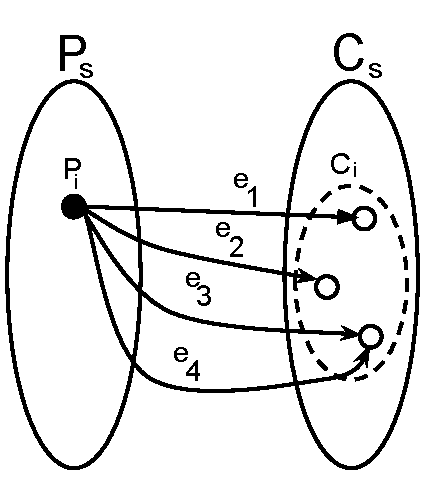
\includegraphics[scale=0.5]{BipartiteGraph.pdf}
            \vspace{5mm}
        \end{figure}
    \end{multicols*}

    \begin{itemize}
        \item[GOAL:]<2-> Are alternate channel implementations worth exploration?
    \end{itemize}

    \inote{
        \item Keep a list of all communications as a graph between set of processes and channels.
    }
\end{slide}

